\documentclass[british,titlepage]{ntnuthesis}

\title{AI in the classroom}
% \shorttitle{TDT4501 Project report Autumn 2024}
\author{Sander Østrem Fagernes \& Fredrik Fonn Hansen}
% \shortauthor{CoPCSE$@$NTNU}
\date{CC-BY \ntnuthesisdate}

\addbibresource{thesis.bib}

\input{glossary.tex} % add glossary and acronym lists before document

\begin{document}

\listoftodos % Remove when done

\tableofcontents
\listoffigures
\listoftables
\lstlistoflistings

\printglossary[type=\acronymtype] % Print acronyms
\printglossary                    % Print glossary

\chapter{Introduction}\label{sec:introduction}

This project report is written as part of the course \textit{TDT4501 - Computer Science, Specialization Project} at the \textit{Norwegian University of Science and Technology} (NTNU) during the autumn semester 2024. The course serves as prepartion for the master's thesis and allows students to gain experience with researching a topic using scientific working methods. We are two Computer science master's students who have carried out the project and authored this report. The project is carried out as preparation for the master's thesis ``AI in the classroom''. Our main supervisor is \textit{Özlem Özgöbek} and our co-supervisor is \textit{George Adrian Stoica}, both associate professors at the department of computer science. We are also collaborating with PhD candidate \textit{Talha Mahboob Alam}. On the side of the project, we have also followed the two theory modules \textit{TDT06 - Educational Technology} and \textit{TDT07 - Learning Analytics} as part of \textit{TDT4506 - Computer Science, Specialization Course}.

The ``AI in the classroom'' master's thesis can be seen as follow-up work from \cite{stoica2016} and \cite{stoica2017}, co-authored by our co-supervisor in 2016 and 2017, respectively. We will come back to these papers in chapter \ref{chap:relatedwork}, but their purpose was to develop a system for visualising open-text responses from students in real-time to provide the instructor with insights. Such a system may be referred to as a classroom response system - among several other synonyms. These systems have a long history, but they have mostly been used with closed-ended questions to gather responses from students, as these are easier to quickly analyse. Closed-ended questions do, however, have several limitations, and both the instructor and the students could benefit from open-ended questions instead that require students to write responses in the form of short text - which we will refer to as ``open-text responses''. While open-text responses can be quickly read through by an instructor in small classrooms, this gets close to impossible in large classrooms or lecture halls. With the development of ever more performant AI and text mining methods, it seems quite likely that such methods can be applied, in combination with a classroom response system and clever visualisations, to help instructors quickly make sense of large amounts of open-text responses in a live class or lecture setting. The investigation into which and how modern text mining methods can be applied to open-text responses to provide instructors with actionable feedback in real-time, as well as the implementation and evaluation of a suitable system, is what defines the master's thesis. In other words, bringing AI into the classroom to improve the learning process.

For the structure of this report, we start by presenting some background for the project and master's thesis in chapter \ref{chap:background}. We will then go through some related work in chapter \ref{chap:relatedwork}. Chapter \ref{chap:method} explains the methods and procedures we have followed for collecting data and performing a systematic  literature review. Chapter \ref{chap:discussion} contains the results of our work and investigation related to data collection, the sytematic literature review, related proprietary solutions, open problems in the domain and planning of the master's thesis itself. To round off, chapter \ref{chap:conclusion} summarises what we have done for this project and the plan ahead for the upcoming semester.







\begin{comment}
The introduction of the thesis should take the reader all the way from the big picture and context of the project to the concrete task that has been solved in the thesis. A nice skeleton for a good introduction was given by \textcite{claerbout1991scrutiny}: \emph{review–claim–agenda}. In the review part, the background of the project is covered. This leads up to your claim, which is typically that some entity (software, device) or knowledge (research questions) is missing and sorely needed. The agenda part briefly summarises how your thesis contributes.
\end{comment}


\chapter{Background}\label{chap:background}


\section{Student engagement and interaction}
\todo{Performance, Læringsutbytte, Studenters motivasjon...}


Interaction and engagement between students and teachers in the classroom is widely perceived as one of the most important factors in learning outcomes, academic performance and general motivation [src]. Additionally, high levels of interaction and engagement often correlate [src] with improved understanding, retention and ability to use the knowledge in other areas. A potential reason to why this happens is that the increased engagement can potentially make learners more connected with the materials. 

Achieving high levels of interactions and engagement can be difficult and resource intensive. In smaller classes, the teacher can often use methods like direct dialogue to communicate and let everyone actively participate throgh questions and discussions. While this is a perfectly good solution, it does not scale well for larger classes. In large classes there is simply not enough time or resources to ensure that every student can contribute one a one-to-one basis. This often leads to a more passive teaching environment [src] with less interaction. This can cause a missed opportunity for effective learning. 

To mitigate these issues, educational technologies like student response systems have been introduced. These systems aims to facilitate direct participation in a classroom through various technology, often through asking real-time questions. One of the main benefits of these digital systems is that the logistical issues of large classes are no longer present. In the following section we will go in more detail through the previous and current solution, and mention benefits and issues with these technologies regarding interaction and learning outcomes. 

% blooms taxonomy
\begin{comment}
    Attendance alone has a low correlation with performance
    Important how the attendence is experienced
    Cognitive engagement partially mediates performance
    Behavourial engagement fully mediates performance
    Tutorials more so than normal lectures
    Flipped classroom and response systems are shown to help engagement in large classes
\cite{Buchele2021}

    
    Challenges:
        Hard to get "just-in-time" feedback from students
        Limited time providing individual feedback
        Limited peer interaction and instructor-learner interaction
        High affective filter when voicing personal views in class
    Benefits:
        Anonymous responses -> Less affective filter, more confident
        Everyone's voice is heard, no one gets to dominate discussion
    Students responded positively to the introduction of a response system
        Great fun, Instantaneous feedback, participation, interaction, independent thinking

    - Bloom’s taxonomy
    - Remember, Understand, Apply → True/False, Multiple-choice
        - Stimulate factual recall
    - Analyse, Evaluate, Create → Item-ranking, open-ended, word-cloud
        - Elicite opinions and views, reveal or challenge misconceptions on a topic

    Word cloud > Brief answers or comments > Item ranking > Multiple-choice
\cite{shi2023}
\end{comment}


\section{Open-ended questions in education}
\todo{Effect of open-ended questions: reflection, critical thinking, bearbeide kunnskap}




\section{Student response systems}
\todo{Move text from 4.1.3 up here about Kahoot and Mentimeter}
\todo{Eksisterende løsninger, og deres drawbacks}
\todo{clickers, kahoot, åpne-spørsmål, live adjustments}
% \cite{resyslitrev}
% https://tophat.com/blog/classroom-clickers/
In this chapter we will go through current and previous solutions that aims to increase student engagement. We will discuss their strengths and weaknesses, as well as potential ideas for improvements that we can build upon.

\subsection{Clickers}
Clickers used in classrooms consists of a combination of hardware and software with the aim of increasing engagement and interactivity. The hardware is typically a combination of remote-controlled devices (similar to a TV-remote), and a receiver that can collect input from the remotes. It usually works by the teacher asking a question to the class, and then each individual can send in the answer. The teacher will usually be able to see the results and can share this with the class, for instance a digital dashboard solution can automatically create graphs and visualizations of how the students have answered. 

Traditional clickers function by using infrared signal to send the response from the remote to the receiver. This can work for smaller classrooms, but large rooms and many students might create ambiguity of wether the response is collected by the receiver (the teacher will be able to see the responses immediately, but the students does not get any feedback. 

Additionally, it is not possible to track answers between questions. Meaning it is not possible to implement things like scores etc...

Clickers can provide engagement and potential for further discussions. It can also make the teacher aware of how the students understand the lecture contents, and can adjust thereafter. 
\todo{Den støtter ikke H, men vi har pakken float installert i Main.tex??}
\begin{figure}[h!]
    \centering
    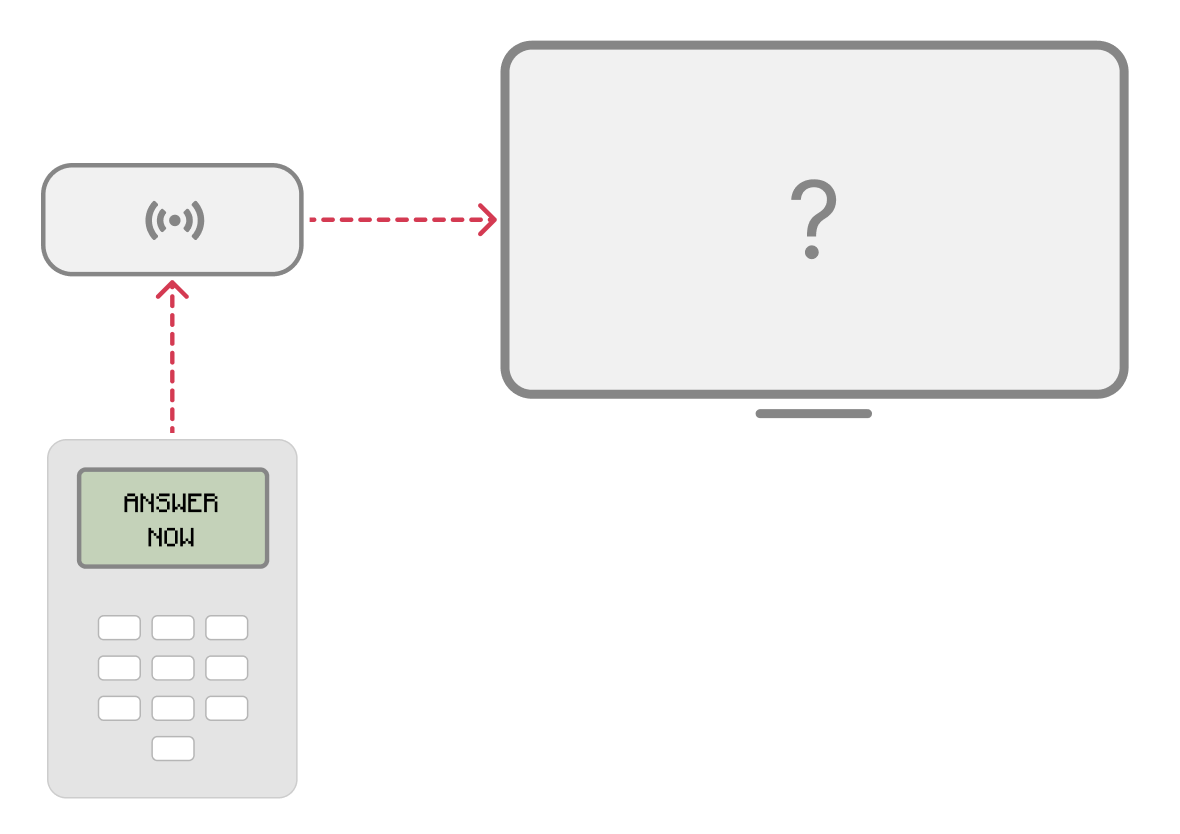
\includegraphics[width=1\linewidth]{figures/clickers-illustration.png}
    \caption{A typical classroom setup with clickers, a receiver and a tv}
    \label{fig:A typical classroom setup with clickers, a receiver and a tv}
\end{figure}


\subsection{Kahoot!}
Kahoot! is a software company that offers a digital solution where students use their mobile phone or computer as the tool for submitting answers.

This approach allows users to join sessions with their custom name and avatar, allowing a more individual approach. On top of this are features like music, leaderboard and scores tools used to further increase the engagement.

By utlizing the internet, the issues with infrared signals are solved, at the cost of requiring a stable internet connection. By utilizing existing hardware (assuming everyone has their own mobile phone), we can drastically reduce the cost of operations for the schools, enabling a more widespread usage. This approach also allows for participating remotely, making participation from digital classrooms and MOOCs possible as well. 

\todo{also mention about open-text grouping}

\begin{figure}[h!]
    \centering
    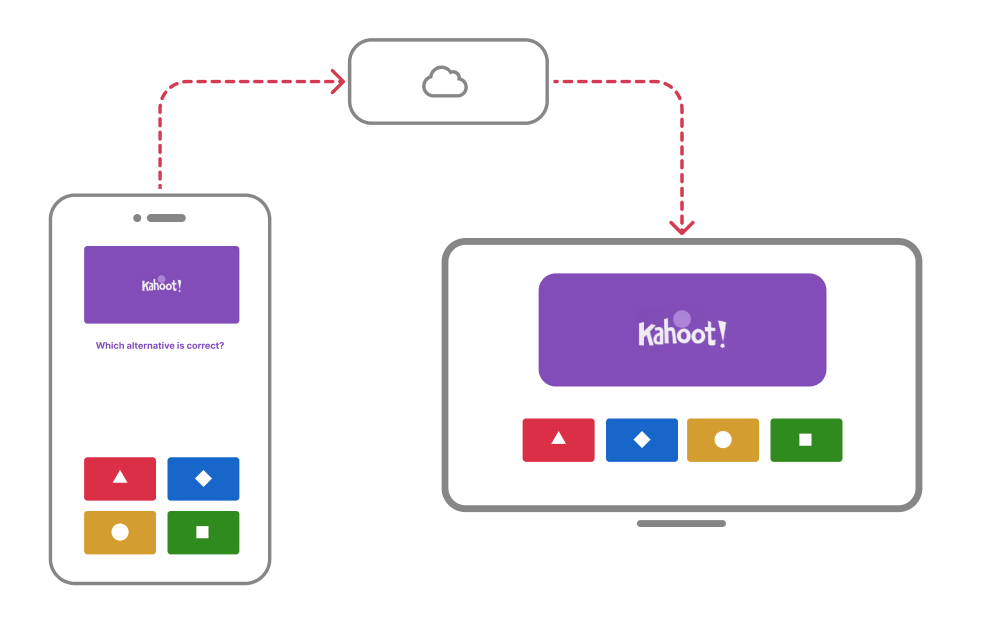
\includegraphics[width=1\linewidth]{figures/kahoot-illustration.png}
    \caption{A Kahoot setup with phones and a tv}
    \label{fig:kahoot}
\end{figure}

\subsection{Mentimeter}
% similar to Kahoot, word-clouds, polls
Mentimeter utilizes similar technology as Kahoot!. It leverages the personal device to connect to a session. 

Mentimeter differs in terms of use context. It has less focus on the gamification, and offers tools like word-clouds and polls.

The polls allow students to vote on different options, and then the graph of distributions will be shown on the screen, allowing students to compare answers. It also has support for other graphs like 1-5 (waves).

Mentimeter also allows users to submit open-text responses, which can be showcased in a word cloud
\todo{might also be able to visualize with boxes? (need to check this out)}
\todo{include images of the actual offering?}

\subsection{Live-questions (traditional)}
% not worth mentioning?
% Can be raise-of-hands as well? 

We have mostly focused on digital solutions, but it can be nice to get an overview of non-digital alternatives.

Raise-of-hands allow the lecturer to ask a question and cast a vote. This can either be yes/no, multiple-choice questions. While this is easy to implement, getting exact measures of distributions might be difficult. In digital classrooms, it might be difficult to get an overview if respondends have low camera quality or poor connection. In large lecture halls it might not be possible to see everyone present from the perspective of the lecturer. 

\section{Challenges with the current systems}
% Move to Discussion part
\todo{Move to discussion part}
% backbround should simply be information that people need to know before reading the thesis

\section{Problem of interpreting open-ended questions}
\todo{Large classrooms, actionable insights}
Interpreting written open-ended answers becomes more cumbersome based on the amount of responses. This usually means that such a system is difficult to use for large classes. 

The time it would take for the lecturer to read and comprehend the responses would take too much focus away from the lecture, potentially reducing the efficiency of the lecture. 

A possible solution could be to have a new role, responsible as administrator of the responses, which role is to read and make optimizations for the lecturer while the lecturer is teaching. However this might cause a weird dynamic, as processes in parallell might take focus away from the learning process.

While smaller classes might make it feasible to read through all responses, it might still be difficult to compare or group responses and make actionable insights. 



% Explain AI, NLP, Text-mining, Sentimental Analysis

% Explain how this can extract themes, gauge sentiment, or detect common misconceptions

% Describe challenges of applying NLP to educational data, such as dealing with informal language, typos, or multilingual responses


\section{Positive impacts of our proposed system}

% Illustrate how AI-driven insights could influence lesson planning or live lecture adjustments, offering concrete examples like identifying misunderstood topics or gaps in student comprehension.

% Discuss how summarization or clustering could help lecturers prioritize feedback on students’ misunderstandings and adapt teaching in real-time.









\begin{comment}
Research projects should always be based on previous research on the same and/or related topics. This should be described as a background to the thesis with adequate bibliographical references. If the material needed is too voluminous to fit nicely in the review part of the introduction, it can be presented in a separate background chapter.
\end{comment}
\chapter{Related work}\label{chap:relatedwork}
% Include concrete papers that have developed some system similar to ours
% Talk about the data used, and why we collected our own

\begin{comment}
    1. What we base our work upon ✅
    2. Use of response systems ✅
    3. Sentiment analysis ✅
    4. Topic modelling + sentiment analysis ✅
    5. SETSUM -> More comprehensive ✅
    6. Assessment and feedback through LLM ✅
\end{comment}

In the papers \cite{stoica2016} and \cite{stoica2017}, Stoica - our co-supervisor - and colleagues present the iLike response system. This system lets the audience - in most cases students - use their own network-connected devices to respond to questions. The goal of the papers was to visualise the open-text responses in real-time in order to use the information in a dialogue with the audience. iLike employs two forms of visualisation of open-text responses. Firstly, a list of all the responses sorted by frequency, which may be useful when the responses are short and many of them are expected to be the same. Secondly, a word cloud showing the most freqeuntly used words. The papers put the most emphasis on the word cloud and highlight a range of challenges with visualising the responses. These challenges include the presence of typos and irregular use of diatcritics in responses, profanities, the repeating of words - referred to as ``shouting'' - common words that are not meaningful - usually referred to as stop-words - and words with similar meaning. The second paper \cite{stoica2017} attempts to deal with some of these challenges through extending the pre-processing pipeline with several filters. It also adds the functionality of drilling into the individual words to see the context within which they originally appear. As the future work outlined by this last paper, in addition to addressing the other identified challenges, incorporating more elements of text mining and natural language processing is mentioned for extracting more meaning from the open-text responses and improve the visualisations. Our work on this master thesis, is part of this future work in incorporating text mining techniques to help instructors make sense of open-text responses in real-time to foster dialogue and engagement in the classroom.

While searching for research on the use of text mining with response systems, we have found a minimal amount of studies. It is, therefore, clear that more research is needed within this domain. One study, however, that addresses this domain is one conducted by Tseng et al. \cite{tseng2018}. They have in their study used topic modelling on open-text responses collected through an instant response system (IRS). They tested three different clustering methods, namely Hierarchical Agglomerative Clustering (HAC), Latent Semantic Analysis (LSA) and Latent Dirichlet Allocation (LDA). Additionally, the developed a processing pipeline which makes use of various rule sets, lexicons and text corpora to deal with punctuation, synonyms, translation when multiple languges are present and for preparing the text for use with the different clustering methods. The paper cannot determine whether any of the three methods are better than the others, and they underline that the presence of many very short text responses hamper the methods' performance and that the choice of which features to extract heavily influences the methods. The paper is only a preliminary exploration of topic modelling used with response systems, so the results are limited. Despite this, the module developed in the study has been used by some instructors in Thailand and Taiwan with the LSA clustering method, where it has proved useful for the instructors. This implies that further research on the use of topic modelling will be valuable. It also provides some evidence that such a system can handle multi-lingual responses. In our case, we will have to handle both English, Norwegian and a mix of both.

Despite limited application of text mining in combination with response systems in the literature, text mining has been applied extensively in the education domain. Neumann et al. \cite{neumann2021} asked in their paper whether sentiment analysis can efficiently measure student emotions from textual feedback and whether the emotions provide instructors with valuable insight. The feedback was collected from students as short unit-of-study reviews related to assignments accompanied by five-star ratings. The paper uses VADER, an unsupervised, rule-based sentiment analysis method. The method consults a lexicon with English terms annotated with sentiment scores to calculate a total sentiment score for a piece of text. They conclude that sentiment analysis provides a more accurate representation of students' emotions than do star ratings - a type of likert-scale response - and that sentiment analysis is a viable alternative to manual reading and labelling of textual reviews, this latter being significantly more time-consuming. The quickness of the feedback also makes it easier for instructors to monitor changes in emotions over time and simple tools, such as word-clouds, can be used to gain insights into why students had a negative or positive feeling about a particular assignment. While the concept of sentiment analysis seems promising, Neumann et al. underlines that the VADER lexicon would require tuning to better match the use-context and that other sentiment analysis methods should be explored.

To gain deeper insight into students' open-text responses, it is also possible to combine different text mining methods. This is what Rääf et al. \cite{raaf2021} have done when analysing learners' reviews from an MOOC. In their study, they start by scraping reviews from the MOOC, cleaning and preprocessing them, and then they combine topic modelling, using LDA, and sentiment analysis, using VADER to assign a sentiment score to each identified topic. This approach makes for more fine-grained sentiment analysis, helping instructors understand what aspects of their courses trigger which emotions in the learners. The study successfully applied the approach to over 30000 MOOC reviews to identify trends and feelings towards five different courses during covid-19. The sample size and context of this study is, however, quite different from what our system would be subjected to, but it shows that combining different text mining can give more fine-grained and meaningful insight. A factor we must keep in mind from this study is that labelling the different topics produced by LDA is done manually, which would not work well in a real-time classroom setting. Some method for automatic labelling must, therefore, be included in our case. The study also outlines that VADER has some difficulty with distinguishing negative texts from neutral ones, most likely due to negation words.

Another example of combining various text mining methods, is the SETSUM system developed by Hu et al. \cite{setsum2022}. The SETSUM system is proposed to provide instructors and higher education management with more in-depth and intuitive reports from Student Evaluations of Teaching (SETs). The analysis of the open-text responses in the SETs is performed by applying sentiment analysis, aspect extraction and extractive summarisation. The system also visualises the results from applying these methods in the final reports using a set of different interactive charts. Differently from the other studies we have looked at, Hu et al. employs machine-learning for the sentiment analysis. This is done in the form of transformer models, more specifically a fine-tuned version of the RoBERTa model. The aspect extraction approach also differs from the topic modelling in the other studies by being weakly supervised. The model is fed with predefined, labelled aspects or topics, each with a set of seed words used to guide the model in assigning open-text responses to the different aspects. This uses a model called Multi Seed Aspect Extractor (MATE). The extractive summarisation method is developed to a greater extent by the researchers themselves. It uses another transformer model, called Sentence-BERT, to create embeddings for each sentence. Then cosine similarity is used to rank the sentences for each aspect. A sentence is then selected by a greedy unsupervised sentence extraction algorithm to take the place as the summary for the given aspect. The system is somewhat complex, but the reports it produces help instructors interpret SET results more efficiently and oftentimes with less bias, according to a survey conducted by the researchers. This study tells us that good visualisations are key, and that combining text mining methods provide more ways for instructors to visualise and udnerstand the information from students' open-text responses. It also goes to show that machine-learning models are viable instruments for open-text analysis in education. However, picking the aspects and seed-words to use requires the context in which the responses are collected to be rather static. This will not be the case for us, as the context of a question asked through a response system will vary dramatically from lecture to lecture and from what insights the instructor wants, such as guaging students' understanding, getting feedback or prompting reflection. Fine-tuning transformer models will also require a lot of data, and how generalisable these models will be is hard to say.

From the public release of ChatGPT in March 2023, the popularity of transformer models has exploded. We have seen in \cite{setsum2022} that finetuned BERT models can be used to interpret open-text responses, but also other language models may be used for this purpose, both through fine-tuning and prompting. Carpenter et al. \cite{carpenter2024} have tested and compared the four large language models, Llama 2, GPT-3.5, GPT-4 and FLAN-T5 in their ability to assess students' explanations to course concepts. The explanations were collected through a response system. The models' prompts were given the instruction of assessing the students' explanations and the question asked. Additionally, the researchers experimneted with including a question-specific assessment rubric, an examplar response created by the teacher, ten labelled student responses to the same question, and combinations of these pieces of information. Due to FLAN-T5's small model size, it was also fine-tuned for each version of the prompt. The task given to the models can be categorised as a multi-class classification task, where they need to label each explanation as correct, partially correct or incorrect. The study found that the fine-tuned FLAN-T5 with the assessment rubric and an examplar response in the prompt performed the best, together with GPT-4 with ten student responses in the prompt. We should keep in mind here that FLAN-T5 is a small-sized open-source model, while GPT-4 is a huge propriatary model that needs to be accessed through OpenAI's API for a per-token fee. Both of these methods require some examples of student responses to the asked questions for them to perform well, FLAN-T5 requires more than GPT-4. This is not necessarily something that is available, especially for ad-hoc questions. Creating the assessment rubrics and examplar responses also adds overhead that may not be feasible in a real-time lecture setting. The paper itself finds that GPT-4 with only the assessment rubric added to the prompt may be the most viable solution for use with a real-time response system.

We see that there are many ways in which text mining methods can be applied to analyse open-text responses in education. Methods can either be used in isolation or several methods can be combined to gain a richer analysis. Both more traditional text mining approaches, such as topic modelling with LDA, and newer approaches using large language models are viable methods, and how we visualise the analysis results is of utmost importance for the usefulness in the eyes of the instructors. While there has been performed little research on text mining in a real-time education setting using response systems, we can undoubtably gain a lot of knowledge and inspiration from literature applying text mining in other education contexts. However, the real-time setting on which we are focusing sets a lot of requirements for our system. We may not have enough data to train or tune machine learning models, there may not be time for the instructor to perform any manual labelling of topics, and the processing must be finished within the span of a few minutes maximum.




\chapter{Method}\label{chap:method}

\begin{comment}
The method chapter should describe in detail which activities you undertake to answer the research questions presented in the introduction, and why they were chosen. This includes detailed descriptions of experiments, surveys, computations, data analysis, statistical tests etc.

Talk about the data used, and why we collected our own
\end{comment}

During the semester, we have carried out a data collection process, a systematic literature review, as well as doing relevant work in the theory modules. We will briefly return to the latter in section \ref{chap:discussion}. The data collection process was conducted to acquire valid data for the development of an AI-driven system next semester. The systematic literature review serves to inform us of previous research and solutions in the field of automated analysis of open-text responses in education. We will present how we carried out these two processes in the following.


\section{Data collection}
To develop an AI-driven system for automatic analysis of open-text responses, it is imperative to have available relevant and valid data. The data will be used for experimentation with different AI methods in the further work with the master thesis.

\subsection{Data requirements}
The final developed system is intended to be deployed into a classroom or lecture hall. This will be done through a response system, where students answer open-ended questions using their laptops or mobile devices. It is, therefore, important that the data be collected in a real class or lecture setting using a response system. This way we can increase the chances of the data having the same quality and nature as the data that will eventually be served to the final system when it is deployed.

To this end, we have defined a set of requirements to which the collected data must adhere for it to be regarded as relevant and valid. The requirements are as follows:

\begin{enumerate}
    \item The data shall be in the form of text
    \item The data shall be produced by humans 
    \item The data shall be produced as responses to questions or tasks through a response system
    \item The data shall be produced in a live class or lecture setting
    \item The data shall be in English, Norwegian or a mix of both
    \item The data shall be anonymised so that individual responses cannot be traced to individual persons
\end{enumerate}

Requirement 1 serves to exclude non-textual responses such as audio, video, answers to multiple-choice questions and votes. It is now, in 2024, not uncommon for text to be produced by generative AI tools or through other computerised means. While a student prompting a generative AI tool to produce a response can provide insight into the student's understanding and sentiment, it is more valuable to have the text produced directly by the student itself. A human writing on a small smart phone screen is also more prone to make typos, write shorter responses and include profanities or slang than generative AI tools, which the final system would need to be able to deal with. As a consequence, requirement 2 restricts responses to be written by humans. This also excludes transcription of human speech. The final AI-driven system will be connected to a response system, where it will in some way aggregate, sort or visualise textual responses to questions or tasks given by an instructor. Requirement 3 mirrors this, and requirement 4 ensures that the data is collected in real-time in an educational context. It will be an important feature of the final system that it can automate the analysis adequately and quickly enough for an instructor to use the analysis for actionable feedback during class or a lecture. Data from, for instance, offline surveys, assessments and discussion forums is not relevant, as students will often have more time to interpret the question or task, formulate the response and the instructor will have more time to understand the analysis, look at individual responses and plan out further action. Moreover, requirement 4 restricts the data to an educational environment. Open-text responses produced through response systems, such as Mentimeter, are used in business environments, as well. However, the initial motivation for this master's thesis is to help instructors interpret open-text responses from their students, and as master students at NTNU, our main contact points are lecturers at the university who can take part in both the data collection and the evaluation of the final system. Language is restricted to English and Norwegian through requirement 5, as these are the two languages we authors master and that are used at NTNU. Both languages are included to avoid ending up with a system that only supports English, enabling us to experiment with multiple languages and language mixing in the responses. Lastly, requirement 6 states that the data must be anonymised. While we can find out which students took part in which lectures, it shall not be possible for us as authors to determine which student wrote which response, in order to protect the students' privacy.


\subsection{Data collection strategy}\label{sec:data-collection-strategy}
To collect the data, we have recruited lecturers at NTNU through a few different fora. This has been done to get recent data collected through student response systems with which we are familiar, and to have the opportunity to include the same lecturers in the evaluation process of the final system. Having our partners close-by to facilitate physical meetings or the opportunity to participate in lectures later to test the final system, has played a role in this choice. It has also proved difficult to find relevant datasets online. The closest related datasets concern survey responses, assessment short answers and MOOC reviews. This is most likely due to these types of data being easier to collect in large numbers compared to open-text responses entered through response systems. Response systems also tend to focus more on other forms of questions instead of open-ended questions.

Before reaching out, we created the question guide poster in appendix \ref{app:question-guide}. The poster contains a short note explaining the purpose of the data collection and our contact information. It then presents three guidelines with examples on how to formulate effective open-ended questions for use in large classrooms or lectures. Lastly, it shows two flow charts depicting the process of preparing a question and the data collection process. The intention of this poster was to hand it out to the lecturers after an initial meeting with them, serving both as a guide on how to formulate the type of open-ended questions we are looking for and as a reminder of how to perform the data collection. Creating the poster was also a way for us to think about which qualities a good open-ended question should possess to help students reflect, learn and provide useful feedback to the lecturer.

In addition to this poster, we wrote the note in appendix \ref{app:recruitment-note}. This note would serve to inform interested lecturers about the goal of our master's thesis, how they could help us collect data and how we could help them in return. The note also encourages lecturers to contact us through the provided contact information if they would be interested in collaborating with us on the data collection.

To reach out to the lecturers, we employed three different fora. Firstly, the aforementioned note was shared on NTNU's intranet, ``Innsida'', by our supervisor. It was here posted under the channel of the faculty of information technology and electrical engineering, under which we and our supervisors belong. Members of the faculty are all in the cross-section of IT and education. This could make it easier for them to understand the purpose of our master's thesis and the utility of the final result. Secondly, the note was shared by our co-supervisor with members of Excited, the Norwegian centre for excellence in IT education. This is an organisation associated with NTNU and Nord university with focus on research on the use of IT in education. We saw this as a relevant point of contact due to our overlapping research field, thinking that they may sit on relevant data or that there would be members who would take interest in the work and want to collaborate. We also held a short presentation for members of Excited about the master's thesis and our need for help with the data collection. The last forum has been direct contact with lecturers through email. Together with our supervisor team, we have reached out to lecturers that we either know use response systems or open-ended questions in their lectures or that teach large classes. In the emails we have described the goal of the master thesis, what data we need and how the lecturer could help, offering to take a short meeting to discuss it.

For each lecturer contacted, we asked both whether they already had anonymised data in the form of open-text responses that they would be willing to share, and whether they would be interested in collaborating with us on collecting more data throughout the semester. In the latter case, we would send them the question guide poster if they thought it would be helpful to them.

\subsection{Data collection tools}
One of the requirements for collecting the data is to do it through a response system. As mentioned in section \ref{sec:responsesystems}, lecturers at NTNU have access to Mentimeter and Kahoot!, both making it possible to ask open-ended questions.

For the lecturers that used Mentimeter, we would get access to the relevant Mentimeter presentations from where we could download the students' responses as .xlsx files. This way it would be less likely that a lecturer or someone else manipulates the results without us noticing, as we get the raw data straight from the source. We did not need to anonymise the responses as Mentimeter never registers any information on the user in the first place. After having downloaded the data, we would notify the lecturer to revoke our access to the Mentimeter presentations. This was done so that we would only have editing access to the presentations in a short time interval to avoid accidental edits and to reassure the lecturers that we could not edit data without them noticing.

In the case of Kahoot!, as each response is connected to a username, the data is not anonymised. We, the authors, shall not have any way of connecting responses to actual students, so the anonymisation of data had to be done by the lecturers before sending the data to us. Kahoot! generates reports in the form of .xlsx files for each Kahoot! session. Of these reports, we are only interested in the type of question - whether it is, for instance, a brainstorming question, open-ended question, multiple-choice question - the question itself, and the text response from the students. We would, consequently, ask the lecturers to send us the data in the report sheet called ``RawReportData Data'' and remove all columns except for the question type, question and answer. We would then receive the data as a .xlsx file over email.

\subsection{Data storage strategy}
While the data is anonymised, it is still to be considered as ``internal'' data according to NTNU's data storage policy. This means that it cannot be stored in cloud services or similar that is not approved by NTNU. Following this, we opted for storing the data in Teams under a team called ``AI in the classroom'' featuring us and the three members of our supervisor team. This would give easy access to the data for the five of us, while respecting rules of NTNU's data storage policy.

\section{Systematic literature review}
As part of the work this semester, we have started conducting a systematic literature review (SLR) in cooperation with a PhD candidate. The SLR is based on the guidelines in \textit{the Preferred Reporting Items for Systematic reviews and Meta-Analyses} of 2020 (PRISMA 2020) \cite{prisma2020}. The work on the SLR will continue the upcoming semester, mainly to be conducted by the PhD candidate, with the end-goal of publishing it. The final paper will follow the exhaustive PRISMA 2020 checklist. This report, however, will only consider a subset of the items in line with the progress made thus far. In this section, we describe the process we have followed in conducting the SLR.

% Describe the rationale for the review in the context of existing knowledge
% Maybe include which literature reviews we have looked at
\subsection{Rationale}
This SLR ties into a greater research effort on utilising modern software tools to leverage the potential in learners' open-text responses in real-time to drive education forwards. Natural language processing has come far in the way of analysing large amounts of unstructured text and generative AI has brought many new opportunities.

In the education domain, the systematic literature review of Gao et al. \cite{autoassessmentlitrev} has looked at the state of automatic assessment systems for text responses in post-secondary education between 2017 and 2023. They synthesised 93 papers, focusing on identifying different types of automatic assessment systems, the learning needs the systems address, the papers' research motivations, the performance of the systems and the future directions in the context of automated text-response assessment. They identified five different systems based on input, processing and output. Input ranged from short text answers from tests, questionnaires and proprietary systems, to written essays and multi-modal input. Output was in the form of numerical scores, labels, visualisations or text in the form of feedback to the students. The processing employed a variety of different AI and natural language processing methods, both supervised, unsupervised and generative AI techniques. Tasks such as semantic similarity, topic modelling and sentiment analysis were included, as well as generating textual feedback through large language models. Being a very recent publication - from 2023 - the review gives us a good idea of which techniques are used to handle open-text responses in education. However, the focus of the review is on assessing students' open-text responses and providing the students with personalised feedback to help them improve, which mainly concerns itself with analysing single student responses. We are, on the other hand, interested in analysing large amounts of student responses together to identify patterns or extract useful information.

A systematic literature review that looks at the analysis of open-text responses more broadly, is that of Takaki \& Dutra \cite{textmininglitrev}. It found 52 papers from 2017 to 2021 that have studied how text mining has been used in distance higher education. 37 of these focus on improving upon traditional teaching by introducing tools to help with the more subjective aspects of teaching, promoting meaningful learning rather than simply automating mechanical tasks. Most of the papers address the instructor's challenge of managing the workload in the face of textual data from a large number of enrolled students, be that in the form of feedback, questions or assessment answers. Some papers focused more on providing students with personalised feedback or guidance or helping management with decision making based on student responses. In terms of text mining tasks, text classification was the most common, followed by sentiment analysis, information extraction, chatbots, topic modelling and semantic similarity. Only a single study tested large language models, which goes to show that the use of generative AI has only recently gained traction these past couple of years. Latent Dirichlet Allocation (LDA) was the single most used text mining method, employed in ten of the papers. The review underlines that the research field of text mining in distance higher education was still in a very early phase, and that the availability of qualified data for text mining in education is lacking, especially in other languages than English. While this review, too, gives us a good pointer to which text mining tasks and methods are employed in education, it limits itself to distance higher education. In our case, it is relevant to expand this domain to also consider secondary education and classes with physical attendance.

This SLR will investigate which and how AI and text mining methods are employed in the broader context of education to make sense of groups of anonymous open-text responses. As Gao et al. \cite{autoassessmentlitrev} have already looked into automatic assessment, this will not be part of this SLR. We will not consider personalised feedback systems either, something that Takaki \& Dutra \cite{textmininglitrev} included in their review. It is important that the open-text responses can be analysed without knowing who wrote it, as tying the analysis to identities would not make the text mining generalisable enough to be used in a response system. With growth of generative AI, our SLR will also be better equipped to investigate how generative AI fares in this research field.

\subsection{Eligibility criteria}
% Specify the inclusion and exclusion criteria for the review and how studies were grouped for the syntheses.
% \begin{itemize}
%     \item Include papers from 2015 to 2024, inclusive
%     \item Include journal articles and conference papers
%     \item Include papers written in English
%     \item Include primary research
%     \item Include empirical studies and experimental setups
%     \item Include papers in the education domain
%     \item Include papers that apply AI to analyse some dataset of written open-text responses and evaluate the applied AI methods
    
%     \item Exclude short papers (posters, keynotes)
%     \item Exclude papers without access to full text
%     \item Exclude papers that are not peer-reviewed
%     \item Exclude papers that rely on the open-text responses being associated with their respective authors
%     \item Exclude papers that solely focus on automatic assessement
% \end{itemize}
In order to guide our selection of papers, we have developed a set of inclusion and exclusion criteria. These are seen in table \ref{tab:eligibilitycriteria}. 

\begin{table}[h!]
\centering
\caption{Inclusion and Exclusion Criteria}
\label{tab:eligibilitycriteria}
\begin{tabularx}{\textwidth}{|X|X|}
\hline
\textbf{Inclusion Criteria} & \textbf{Exclusion Criteria} \\
\hline
IC1: Include papers from 2015 to 2024, inclusive & EC1: Exclude short papers \\
\hline
IC2: Include journal articles and conference papers & EC2: Exclude papers without access to full text \\
\hline
IC3: Include papers written in English & EC3: Exclude papers that are not peer-reviewed \\
\hline
IC4: Include primary research & EC4: Exclude papers that rely on the open-text responses being associated with their respective authors \\
\hline
IC5: Include empirical studies and experimental setups & EC5: Exclude papers that solely focus on automatic assessment \\
\hline
IC6: Include papers in the education domain & \\
\hline
IC7: Include papers that apply AI to analyse some dataset of written open-text responses and evaluate the applied AI methods & \\
\hline
\end{tabularx}
\end{table}

\subsection{Information sources}
% Specify all databases, registers, websites, organisations, reference lists and other sources searched or consulted to identify studies. Specify the date when each source was last searched or consulted.
To search for papers, we have both searched scientific literature databases and performed one iteration of forwards and backwards snowballing. The databases searched were \textit{Web of Science}, \textit{Scopus}, \textit{ACM Digital Library}, \textit{Proquest} and \textit{ERIC}. The search was carried out October 21st 2024. For the snowballing, we looked into the citations and references of all papers from the database search that were still included after full text screening. \textit{Google Scholar} was used to find and retrieve these papers if not directly reachable through a DOI. Snowballing was performed in the period from the 31st of October to the 16th of November 2024.

\subsection{Search strategy}
% Present the full search strategies for all databases, registers and websites, including any filters and limits used.
To search the databases for relevant literature, we developed this search query

\begin{quote}
    \textit{(``text*'' OR ``response*'' OR ``answer*'' OR ``question*'') AND ((``teacher*'' OR ``instructor*'' OR ``educator*'') AND (``student*'' OR ``learner*'')) AND (``in-class'' OR ``classroom*'' OR ``lecture*'') AND (``artificial intelligence'' OR AI OR ``machine learning'' OR ML OR ``text mining'' OR ``data mining'' OR ``text analy*'' OR ``language processing'') NOT (grading OR scoring)}
\end{quote}

We used this query for all five databases, but had to change \textit{NOT} to \textit{AND NOT} in Scopus. The search query is made up of a few different components connected by the logical keywords \textit{AND}, \textit{OR} and \textit{NOT}. Table \ref{tab:searchquery} explains why these components are included. The asterisk is a wildcard that, here, mainly ensures that both the singular and plural forms of the words are part of the search.

\begin{table}[h!]
\centering
\caption{Database search query composition}
\label{tab:searchquery}
\begin{tabularx}{\textwidth}{|X|X|}
\hline
\textbf{Component} & \textbf{Purpose} \\
\hline
(``text*'' OR ``response*'' OR ``answer*'' OR ``question*'') & There are too many terms used for open-text responses to include them all. We, therefore, opt for these four more general terms \\
\hline
((``teacher*'' OR ``instructor*'' OR ``educator*'') AND (``student*'' OR ``learner*'')) & Anchor papers in education. Ensure that both instructors and learners are addressed, as we are interested in the interaction between these two parties \\
\hline
(``artificial intelligence'' OR AI OR ``machine learning'' OR ML OR ``text mining'' OR ``data mining'' OR ``text analy*'' OR ``language processing'') & Ensure that papers address the use of AI. We include some synonyms with emphasis on applying AI to text \\
\hline
(grading OR scoring) & Exclude papers focusing on automatic assessment \\
\hline
\end{tabularx}
\end{table}

We performed the search over the papers' titles, abstracts and keywords to avoid getting too many irrelevant results due to matches in the papers' full texts. The option for which parts of the papers to search differed somewhat, however, between the databases. We also set other filters and limits for the searches in line with our eligibility criteria. In some cases we included more document types than just journal articles and conference papers, but these were excluded during later screening. All the filters and limits are presented in table \ref{tab:filtersandlimits}.

\begin{table}[h!]
\centering
\caption{Database search filters and limits}
\label{tab:filtersandlimits}
\begin{tabularx}{\textwidth}{|X|X|X|X|X|X|}
\hline
\textbf{Database} & \textbf{Within} & \textbf{Year} & \textbf{Language} & \textbf{Type} & \textbf{Other} \\
\hline
Web of science & Topic & 2015-2024 & English & Papers, conference proceedings, review articles, early access & \\
\hline
Scopus & Article title, Abstract, Keywords & 2015-2024 & English & Conference paper, article, book chapter, conference review, book, review & \\
\hline
ACM Digital Library & Abstract & 2015-2024 & English & Research article & \\
\hline
Proquest & Anywhere except full text - NOFT & 2015-2024 & English & Article, feature, conference proceedings, review & Full text, Peer reviewed \\
\hline
ERIC & abstract: & 2015-2024 & & Journal articles & Full text available on ERIC, Peer reviewed only \\
\hline
\end{tabularx}
\end{table}


\subsection{Selection process}\label{sec:slr-selection-process}
% Specify the methods used to decide whether a study met the inclusion criteria of the review, including how many reviewers screened each record and each report retrieved, whether they worked independently, and if applicable, details of automation tools used in the process.
The selection process consisted of several steps of searching and screening.

\begin{enumerate}
    \item \textit{Database search}: We first input our search query into the five scientific literature databases and applied the filters and limits described in table \ref{tab:filtersandlimits}. The resulting papers were extracted to Endnote and Endnote was used to remove duplicate papers. The publication type, authors, publication year, title and abstract of each paper were at last exported from Endnote to an Excel document.
    \item \textit{Abstract screening}: Before going through the full text of each paper, we applied the eligibility criteria to the titles and abstracts of the papers in the Excel document. The amount of papers were split in half between the PhD candidate and one of us, marking each paper as either ``Included'' or ``Excluded''. We did not provide an exclusion reason at this stage. In case of uncertainty, the paper would be included for more scrutiny in the next phase.
    \item \textit{Full text screening}: The papers included in the abstract screening, were copied to a new Excel sheet, again splitting the amount of papers between the same two people. The eligibility criteria were now applied to the full text. A reason was provided for why papers were excluded, and if one of us were uncertain about a paper, the other would go through it, as well.
    \item \textit{Snowballing}: For any papers included after full text screening, we performed a single iteration of forwards and backwards snowballing. Forwards snowballing was done by going through the papers' citations and backwards snowballing by going through their references. In each case, we first applied the eligibility criteria to the titles. We then applied them to the abstracts of the papers whose titles fulfilled the criteria. After going through the relevant abstracts, the included papers would be added to yet another Excel sheet.
    \item \textit{Snowballing full text screening}: We would then repeat the full text screening for the papers found during snowballing.
\end{enumerate}

After concluding the selection process, the papers left after full text screening of the papers from both the database searches and the snowballing, were collected in a new Excel document ready for data extraction. Any duplicate papers not removed by Endnote would also be removed before this.

\subsection{Data collection process}
% Specify the methods used to collect data from reports, including how many reviewers collected data from each report, whether they worked independently, any processes for obtaining or confirming data from study investigators, and if applicable, details of automation tools used in the process
To extract data from the included papers, we had a row for each paper in an Excel sheet. The columns represented different categories of data, with each cell containing one or more codes and optionally a comment in parentheses behind each code to add context or reasoning. The selected columns were based on the rationale for this SLR, but we also used the columns from \cite{autoassessmentlitrev} and \cite{textmininglitrev} as inspiration. The initially selected columns were

\begin{itemize}
    \item Title of work
    \item Author(s)
    \item Year
    \item Journal/Event
    \item DOI
    \item Abstract
    \item Research motivation
    \item Educational domain
    \item Educational level
    \item Learning environment
    \item Target population
    \item Educational theories
    \item Data source
    \item Data language(s)
    \item Dataset size
    \item AI tasks
    \item Preprocessing
    \item Number of algorithms used
    \item Tools
    \item Validation method
    \item Evaluation metrics
    \item Evaluation results
    \item Educational benefits
    \item Limitations
    \item Future directions
\end{itemize}


For the codes, we employed an open coding approach, where we developed the codes as we read through the papers. Each code would be added to a table in a separate Excel sheet for reference with an accompanying description. We started out with rather fine-grained codes, which were subsequently discussed and later merged where applicable. The data extraction was carried out by three people - the same two as did the screening in addition to another one of us authors. We read through and coded a third of the papers each.

The current results from the SLR will be reported in section \ref{sec:results-slr}. There, we will also explain the current status of the SLR and the way forwards.
\chapter{Discussion}\label{sec:discussion}

\begin{comment}
The results chapter should simply present the results of applying the methods presented in the method chapter without further ado. This chapter will typically contain many graphs, tables, etc. Sometimes it is natural to discuss the results as they are presented, combining them into a `Results and Discussion' chapter, but more often they are kept separate.

Here you should discuss all aspect of your thesis and project. How did the process work? Which choices did you make, and what did you learn from it? What were the pros and cons? What would you have done differently if you were to undertake the same project over again, both in terms of process and product? What are the societal consequences of your work?

IT2810 - Web development
IT3021 - Game+
TET4205 - Power system analysis 2
IT3402 - Service design
Trond Morten

Innsida - Two reached out, one provided data
Excited - No response
Contact persons - 3
Co-supervisor contact - 1
Backup - Peer reviews

Do we have enough data?
\end{comment}

\section{Collected data}
% Write about what we know about the data. In the final thesis, have a more in-depth analysis

As described in section \ref{sec:data-collection-strategy}, we have reached out to potential collaborators through a few different channels with the goal of collected open-text responses submitted by students through a response system.

Firstly, our attempt at reaching out to the members of Excited did not yield any result. As for the note published on Innsida, we had two lecturers reach out to us. One of them, a lecturer of an electrical engineering course, has collected open-text responses through Mentimeter this semester at regular intervals and shared the responses with us. The obtained dataset contains various types of questions, such as multiple-choice and scales, but also open-text questions. There are in total 337 responses, as of September 19th, written in English. The length varies from a single word to a couple of short sentences. The amount may increase if we receive the responses from the second half of the semester.

In terms of lecturers we have reached out to directly, we have received responses from three, all within the domain of computer science. Two of the datasets are quite small. The first of them consists of 24 Norwegian responses distributed over three questions. The second consists of eight responses in Norwegian also distributed over three questions. Both datasets are collected through Mentimeter. These two datasets are hardly large enough to be of much use, as it is easy for a lecturer to look through all the responses to a question during a lecturer; there is no need for any computer-assisted analysis of the responses. The third dataset, on the other hand, is more extensive. It contains 15 questions with 478 English responses with between 19 and 43 responses per question. The responses vary from a single word to a short sentence. An interesting feature of this dataset is that some responses contain emojis, which is something that our system must handle.

The last collected dataset was shared with us by a contact of our co-supervisor. They are also a lecturer at NTNU, and the dataset contains around 1000 responses collected over a few years in engineering courses. The responses are mainly in Norwegian. We are currently not in possession of the dataset, but we will receive it before starting experimentations next semester.

In conclusion, we have managed to collect three datasets of sufficient size - around 1800 responses - and a sufficient number of responses per question for them to be valuable during experimentation with AI methods. We also have both English and Norwegian responses. At this point in time, we have not yet analysed the datasets. In the final master thesis, we will include a thorough analysis of the collected datasets.

\section{Systematic literature review}\label{sec:results-slr}
% Talk about the plans for the SLR for the next semester
% Mention resources, search string, number of results, exclusions
In this section, we will present the results we have thus far from our SLR. We will also explain what is missing at this point in time and lay out the road ahead for the upcoming semester, spring 2025.

\subsection{Study selection}
% Describe the results of the search and selection process, from the number of records identified in the search to the number of studies included in the review, ideally using a flow diagram
Following the selection process outlined in section \ref{sec:slr-selection-process}, we obtained the results as shown in the PRISMA flowchart of figure \ref{fig:prisma-flowchart}.

\begin{figure}[h!]
    \centering
    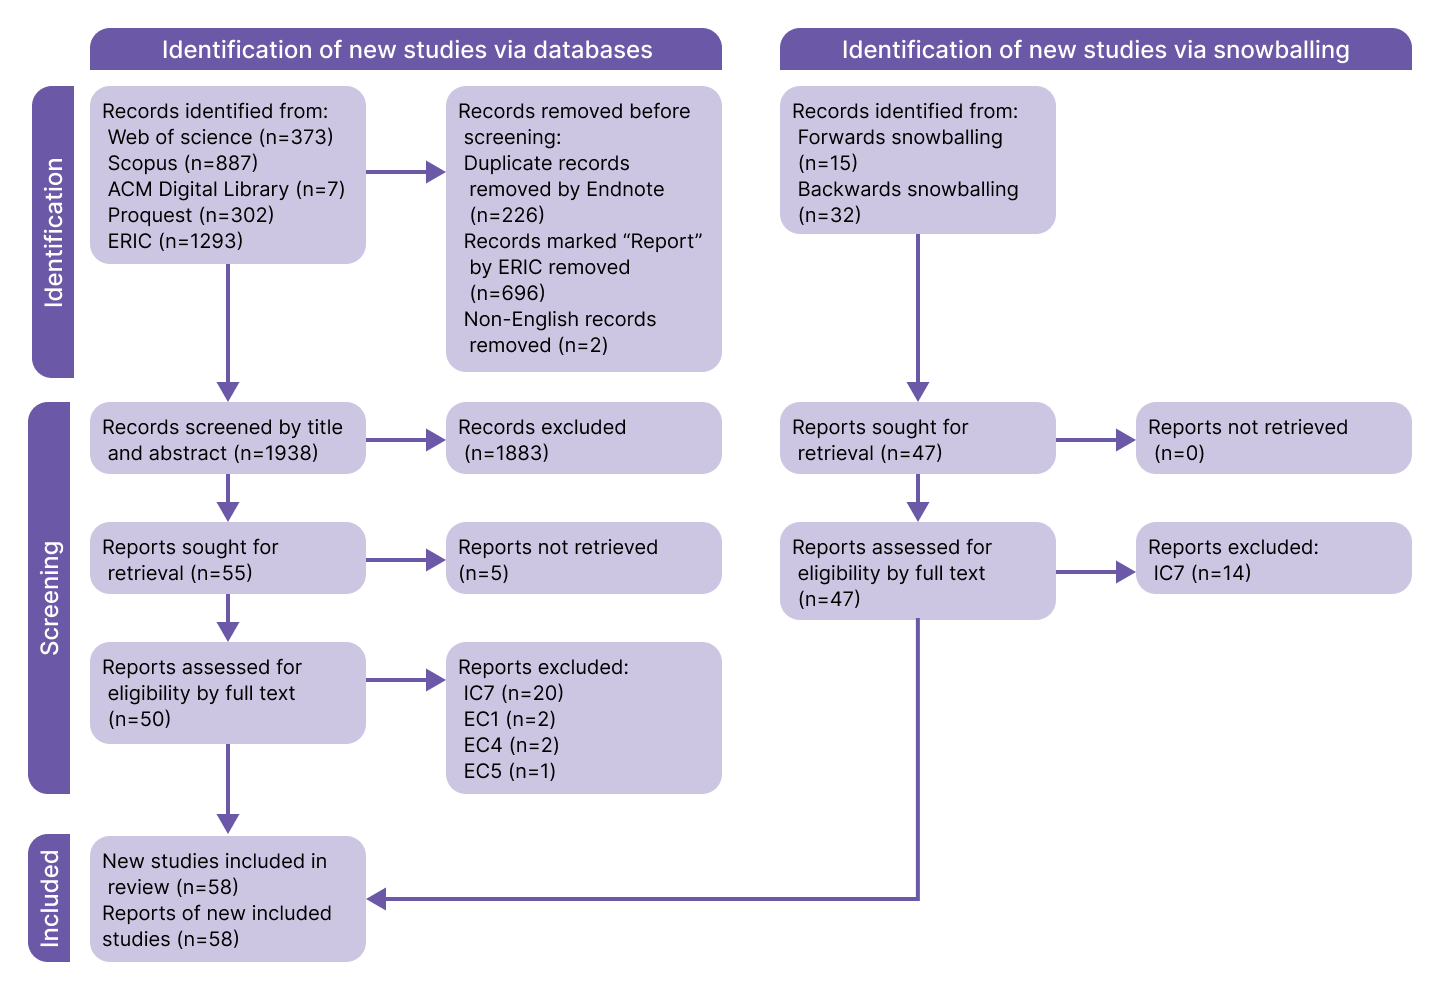
\includegraphics[width=\textwidth]{figures/PRISMA diagram.png}
    \caption{PRISMA flowchart depicting the results of the study selection process.}
    \label{fig:prisma-flowchart}
\end{figure}

When we entered our search query into the five scientific databases and applied the respective filters and limits, we ended up with a total of 2862 papers. 373 of these came from Web of science, 887 from Scopus, only seven from ACM Digital library, 302 from Proquest and 1293 from ERIC. After having exported all the papers to Endnote, we noticed that 696 of the papers coming from ERIC were marked as reports instead of journal articles, despite having set the \textit{Journal articles} filter. These were removed, as we are interested in paper describing new research. After that we used Endnote's built-in functionality to remove duplicates, which resulted in 226 fewer papers. Lastly, two papers were removed that were not in English, leaving us with 1938 papers for screening.

When screening the titles and abstracts, we applied the eligibility criteria. 1883 papers were excluded after this, leaving 55 papers. Five of these did not have full text available. 50 papers were subsequently full text screened and the exclusion reason reported. For the IDs of the eligibility criteria refer to table \ref{tab:eligibilitycriteria}.

We, thereafter, performed an iteration of forwards and backwards snowballing on the 25 papers that were included after full text screening. 15 papers were found through forwards snowballing, which is to say through the papers' citations, and 32 through backwards snowballing, which is to say through the papers' references. Some papers appeared both in citations and references, in which case they are reported as coming from backwards snowballing. Papers that were already found through searching the databases were immediatly excluded as duplicates and not part of the reported statistics in figure \ref{fig:prisma-flowchart}. Snowballing resulted in 47 new papers, of which 14 were excluded due to them not fullfilling inclusion criterion IC7. We were then left with 33 papers from snowballing, with the total count of included papers being 58. These 58 went on to be part of the data extraction process.

While these 58 papers are all published in the period 2015-2024, we have compiled the bar chart in figure \ref{fig:papersbyyear} to get an idea of the papers' timeline. Most of the papers were published in 2019, 2023 and 2020. However, the chart shows no significant trend.

\begin{figure}[h!]
    \centering
    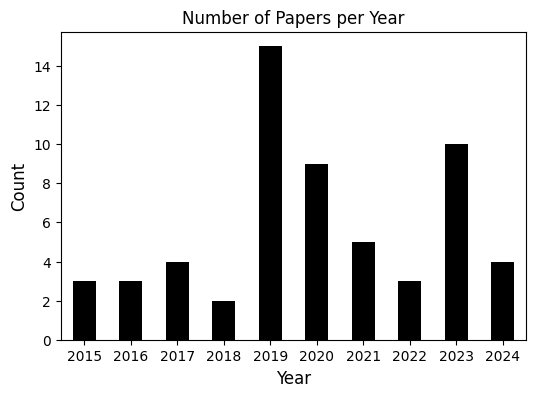
\includegraphics[width=\linewidth]{figures/papers-by-year.png}
    \caption{Distribution of included papers by publication year}
    \label{fig:papersbyyear}
\end{figure}

\subsection{Current status}
As mentioned, the work on the SLR is not completed and will resume in the spring semester 2025, with the aim of publishing it eventually on the side of the master thesis. At this point in time, we have completed the study selection, and we have carried out data extraction for the 58 included papers. The data extraction still requires some work, however. We will in the following attempt to explain the next steps for the SLR.

\begin{enumerate}
    \item \textit{Quality assessment}: The quality of the included papers must be assessed. For this we must develop some quality assessment rules to be applied on all 58 papers. This will ensure that the papers contain sufficient information for our needs and that the results of the studies are truly relevant for our SLR.
    \item \textit{Research questions}: While we have an outline for what data shall be reported in the SLR and an idea of what the SLR should accomplish, we still need to define concrete research questions that can be answered during sythesis of the results.
    \item \textit{Continue data extraction}: We have already extracted data from all 58 papers, but the codes need to be refined further to make the reporting of the data more meaningful and valuable.
    \item \textit{Data synthesis}: After reporting the extracted data, we must make sense of the findings and use the insight to answer our research questions.
    \item \textit{Write the paper}: When we have answered our research questions, the paper itself must be written. This will include explaining the rationale of our SLR, present our research questions and why they are relevant, present the employed SLR methodology, report the results of the paper selection process, report the data from the included papers, answer the research questions, and conclude on what we have achieved with the SLR.
\end{enumerate}

Until now we have been three people working on this SLR. This includes the two of us - in the form of two master students - and a PhD candidate. In the coming semester, the work will mainly be conducted by the PhD candidate while we focus on the master thesis. To perform our experiments on the collected open-text data next semester, we will be dependent on using insights from the SLR as a guide in choosing which AI methods to test, which preprocessing steps and tools may be effective and how different AI methods can be combined to provide more actionable insights from the open-text data.

\subsection{Main findings from papers}
\todo{Describe which AI algorithms have been used, how data was collected and results}

\section{Proprietary solutions}
In addition to consulting literature, we have looked into how the two response systems, Mentimeter and Kahoot!, use AI to analyse open-text responses.

Mentimeter provides two options for analysing open-text responses using AI. The summary feature can be used for the open-ended and word-cloud question types. After a few seconds of processing, Mentimeter will provide a summary in the form of a handful of key points, each around five words with a suitable emoji. The summary feature is briefly explained in \cite{mentisummary}. The grouping feature, explained in \cite{mentigrouping}, can be used for the open-ended question type. If a question has more than ten responses, they can be grouped according to themes. Labels are automatically assigned to each group, and the user can select a group to see the related responses. Except for explaining these features themselves, Mentimeter does not provide any information on how they are implemented, however.

Kahoot! uses AI for clustering ideas submitted in response to their brainstorming question type. One of the developers at Kahoot!, who took part in implemented the clustering algorithm, explains how it works in \cite{kahootclustering}. He explains here that they have chosen an unsupervised clustering method. It uses the \textit{xlm-r-bert-base-nli-stsb-mean-tokens} model from the \textit{Sentence Transformers} Python library to create embeddings for the open-text responses. These embeddings are vector representations optimised for comparing semantic similarity between pieces of text. They then use a classical clustering method - he mentions \textit{K-means} in the article - and follow the \textit{elbow method} with a few optimisations to choose the appropriate number of clusters. As they had performance problems due to high dimentionality, they applied the \textit{TruncatedSVD} module from the \textit{scikit-learn} library to reduce it. While this algorithm has worked well, the article, which is from 2022, underlines that updates are in order. Newer transformer models have been made available and should be tested, auto-encoders should be explored to help reduce dimentionality of the embeddings, and other clustering algorithms should be checked out, such as \textit{HDBSCAN} and \textit{FAISS}.

All of these features are tried and tested in practice, which goes to show that real-time analysis of open-text responses through response systems is, indeed, viable. While Mentimeter and Kahoot! have implemented clustering and summarisation, we intend to look into more methods, such as sentiment analysis, as well as whether methods can be combined.

\section{Open problems in the domain}
\todo{What future research is needed in the field?}




% Keep preliminary RQ as a goal instead of finding a concrete RQ

% \section{Preliminary research question for master thesis}
% \todo{Create a research question for next semester based on the findings}

% Suggestion: How to get actionable insights from students' open-text responses through the use of AI?
\chapter{Conclusion}\label{sec:conclusion}

% Keep very short about we have done in this report
% Paragraph about what we will do next semester

\begin{comment}
The conclusion chapter is usually quite short – a paragraph or two – mainly summarising what was achieved in the project. It should answer the \emph{claim} part of the introduction. It should also say something about what comes next (`future work').
\end{comment}


\section*{\bibname}
\printbibliography[heading=none]

% \input{chapters/papers.tex}

\appendix
\chapter{Question guide}\label{app:question-guide}

The question quide in the form of the poster below, would be sent to instructors agreeing to collaborate on data collection. It would serve as a reminder of the data collection process entails and as a quide on how to create suitable open-ended questions that will harvest insights from the students' open-text responses during lectures. The poster was, however, only sent to two lecturers; most had experience with asking open-ended questions and did not feel the need for having the poster as a reminder or guide.

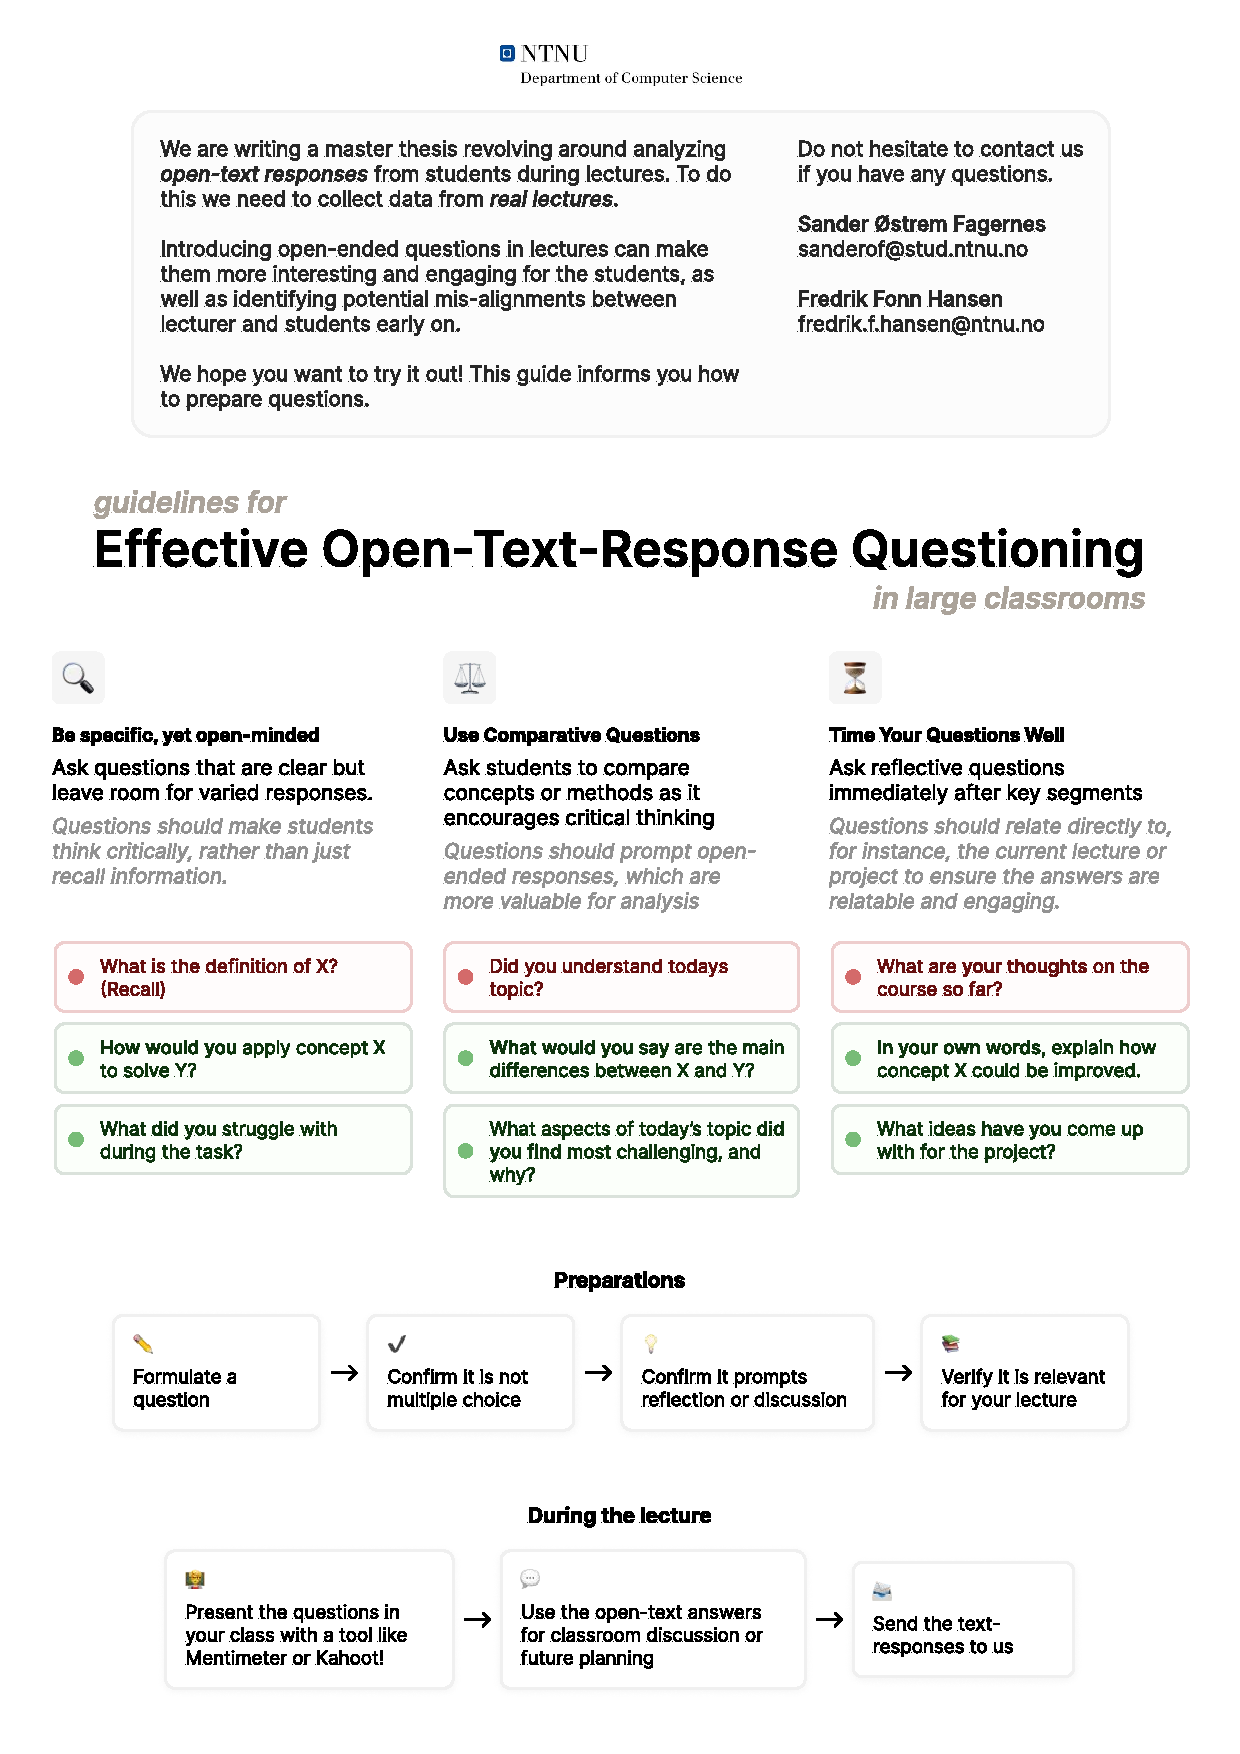
\includepdf[pages=-]{appendices/Question-guide-poster.pdf}
\chapter{Recruitment note}\label{app:recruitment-note}

The following note was shared by us in collaboration with out supervisor and co-supervisor on the NTNU intranet, ``Innsida'', and with members of EXCITED. The purpose was to recruit instructors to help us collect open-text responses from their students.

\setlength\parskip{1em plus 0.1em minus 0.2em}
\setlength\parindent{0pt}

\section*{Looking for teachers to support the ``AI in the classroom'' master's thesis}

\textbf{We are looking for teachers to support the "AI in the classroom" master's thesis. In return we are hoping to help you to support you in your lectures. If you are already using interactive tools in your lectures, you could help us by sharing the anonymized open text answers from your students. More details and contact information is below.}

\textbf{Are you looking to boost student engagement and deepen learning outcomes in your courses?}

We are two students working on our master's thesis focused on improving in-classroom interactivity using open-ended questions. We are seeking lecturers interested in exploring this approach and collaborating with us on our research.

\textbf{Purpose of Our Master Thesis}

\begin{itemize}
    \item \textbf{Enhancing Interactivity and Reflection:} Open-ended questions encourage students to reflect more deeply, leading to more thoughtful responses and honest feedback.
    \item \textbf{Real-Time Challenges:} We recognize that interpreting numerous open-text responses during a lecture can be challenging.
    \item \textbf{Our Goal:} To analyze and experiment with these open-ended responses to develop effective strategies for real-time interpretation and feedback.
\end{itemize}

\textbf{Value for You as a Lecturer}

\begin{itemize}
    \item \textbf{Increase Engagement:} Implementing open-ended questions can make your lectures more interactive.
    \item \textbf{Early Misconception Detection:} Identify and address student misunderstandings promptly.
    \item \textbf{Insightful Feedback:} Open-ended responses may provide you with valuable feedback to improve your course.
\end{itemize}

\textbf{What Participation Involves}

\begin{itemize}
    \item \textbf{Incorporate Questions:} Integrate a few open-ended questions into your lectures that require 2-5 minutes for students to answer.
    \item \textbf{Collect Responses:} Use tools like Mentimeter or Kahoot to gather anonymous student responses.
    \item \textbf{Use the responses:} Optionally use the insight to adapt or improve your lectures in real-time.
    \item \textbf{Share Data:} Email the collected responses to us.
\end{itemize}

\textbf{Next Steps}

If this collaboration interests you, please contact us. We would be delighted to arrange a meeting at your convenience to discuss details — without any obligation on your part.

Your participation would not only contribute significantly to our research but also potentially enhance your teaching practice.

Best regards,

Sander Østrem Fagernes (sanderof@stud.ntnu.no)

Fredrik Fonn Hansen (fredrik.f.hansen@ntnu.no)

\setlength\parskip{0pt plus 1pt}
\setlength\parindent{15pt}

\end{document}
